\documentclass{beamer}
\usepackage[utf8]{inputenc}

\title{Project 1}
\subtitle{Data Analysis of Monte Carlo Simulation of InGAs Semiconductor Device}
\author{Michael Brunetti}
\institute{
EECE 5090 -- Linear Systems Analysis\\
UMass Lowell}
\date{May 28, 2019}
 
 
 
\begin{document}
 
\frame{\titlepage}

\begin{frame}{Strategy}
    \begin{itemize}
        \item Visual analysis
        \item Noise reduction -- fourth-order Butterworth filter with $f_{3\textnormal{dB}} = 500 \textnormal{ GHz}$
        \item Least squares fit, model function: $I = I_{ss} + A e^{-t/\tau} cos \left( 2 \pi f t + \phi \right)$
        \item Analyze voltage vs steady-state current ($I_{ss}$)
    \end{itemize}
\end{frame}
 
\begin{frame}{Device 1 -- Visual Analysis}

\begin{columns}
\begin{column}{0.5\textwidth}
\begin{figure}
    \centering
    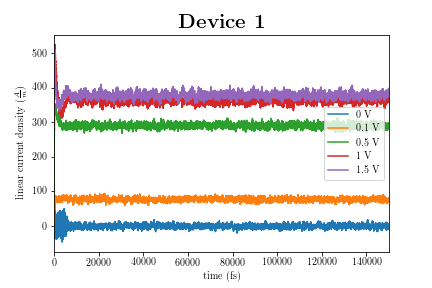
\includegraphics[scale=0.35]{Figures/Device_1/0_to_1_5.png}
    \label{fig:dev_1_1}
\end{figure}{}
\end{column}

\begin{column}{0.5\textwidth}
\begin{itemize}
    \item 0 V, AWGN noise, $\textnormal{mean} = 0 \frac{\textnormal{A}}{\textnormal{m}}$, $\sigma = 4.72 \frac{\textnormal{A}}{\textnormal{m}}$
    \item Response looks second order
    \item Steady-state value with decaying oscillations
    \item Steady-state saturation at $V \geq 1 \textnormal{ V}$
\end{itemize}
\end{column}
\end{columns}

\end{frame}

\begin{frame}{Device 1 -- Visual Analysis}

\begin{figure}
    \centering
    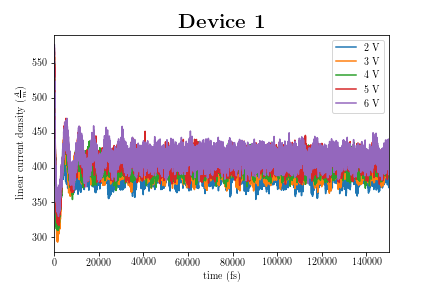
\includegraphics[scale=0.5]{Figures/Device_1/2_to_6V.png}
    \label{fig:dev_1_2}
\end{figure}

\end{frame}

\begin{frame}{Device 1 -- Visual Analysis}
\begin{figure}
    \centering
    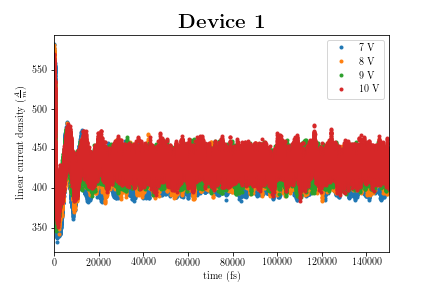
\includegraphics[scale=0.5]{Figures/Device_1/7_to_10V.png}
    \label{fig:dev_1_3}
\end{figure}
\end{frame}

\begin{frame}{Device 1 -- Least Squares Fit}
    \begin{table}[]
        \centering
        \begin{tabular}{c|c c c c c}
            Potential (V) & $I_{ss} \left( \frac{A}{m} \right)$ & $A \left( \frac{A}{m} \right)$ & $\tau (fs^{-1})$ & $f ({GHz})$ & $\phi$ \\
            0.0V & 0.019 & 2.535 & 21485.326 & 23.79e & 0.090 \\
            0.1V & 77.114 & 150.177 & 1445.860 & 28.13e & 14.427 \\
            0.5V & 290.489 & 121.998 & 1381.979 & 161.2 & -27.486 \\
            1.0V & 362.484 & 69.103 & 4599.648 & 146.7 & -38.298 \\
            1.5V & 378.867 & 47.094 & 4530.814 & 152.5e & -31.200 \\
            2.0V & 386.603 & -50.277 & 3147.451 & 168.9 & -27.532 \\
            3.0V & 396.042 & -109.606 & 3960.664 & 167.6 & -21.091 \\
            4.0V & 402.939 & 101.358 & 4759.568 & 163.8 & 0.906 \\
            5.0V & 408.584 & -83.844 & 6970.881 & 162.7 & -21.166 \\
            6.0V & 413.809 & 61.526 & 11258.244 & 162.8 & 5.544 \\
            7.0V & 417.989 & -68.995 & 10213.410 & 155.8 & 3.838 \\
            8.0V & 422.669 & 67.139 & 7408.109 & 141.7 & 5.441 \\
            9.0V & 427.040 & 60.321 & 5789.370 & 140.9 & 1.054 \\
            10.0V & 430.729 & -50.401 & 9899.451 & 138.0 & -27.394 \\
        \end{tabular}
        \label{tab:dev_1}
    \end{table}
\end{frame}

\begin{frame}{Device 1 -- Least Squares Fit}
    \begin{figure}
        \centering
        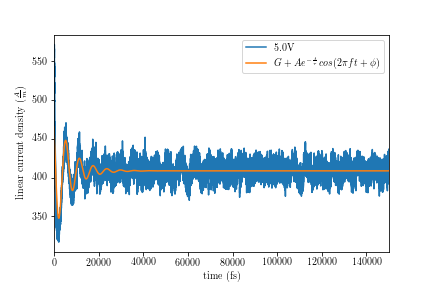
\includegraphics[scale=0.5]{Figures/Device_1/Curve_fit/5_0V.png}
        \label{fig:dev_1_lsq}
    \end{figure}
\end{frame}

\begin{frame}{Device 1 -- Channel Voltage vs Steady-State Current}
\begin{figure}
    \centering
    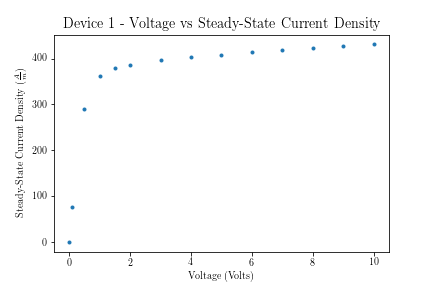
\includegraphics[scale=0.5]{Figures/Device_1/SteadyState.png}
    \label{fig:dev_1_steady}
\end{figure}
\end{frame}
 
\begin{frame}{Device 2 -- Visual Analysis}

\begin{columns}
\begin{column}{0.5\textwidth}
\begin{figure}
    \centering
    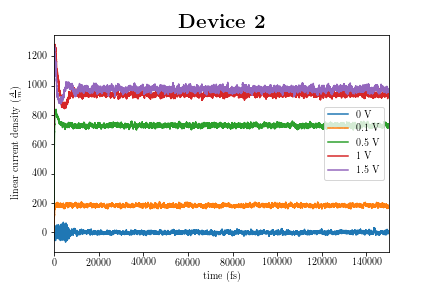
\includegraphics[scale=0.35]{Figures/Device_2/0_to_1_5.png}
    \label{fig:dev_2_1}
\end{figure}{}
\end{column}

\begin{column}{0.5\textwidth}
\begin{itemize}
    \item 0 V, AWGN noise, $\textnormal{mean} = 0 \frac{\textnormal{A}}{\textnormal{m}}$, $\sigma = 6.95 \frac{\textnormal{A}}{\textnormal{m}}$
    \item Response looks second order
    \item Steady-state value with decaying oscillations for $V \leq 8 \textnormal{ V}$
    \item Sustained oscillations for $V \geq 9 \textnormal{ V}$
    \item Steady-state saturation at $V \geq 1 \textnormal{ V}$
\end{itemize}
\end{column}
\end{columns}

\end{frame}

\begin{frame}{Device 2 -- Visual Analysis}

\begin{figure}
    \centering
    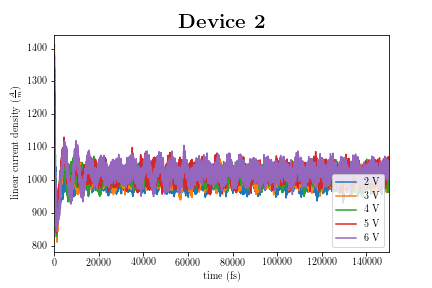
\includegraphics[scale=0.5]{Figures/Device_2/2_to_6V.png}
    \label{fig:dev_2_2}
\end{figure}

\end{frame}

\begin{frame}{Device 2 -- Visual Analysis}
\begin{figure}
    \centering
    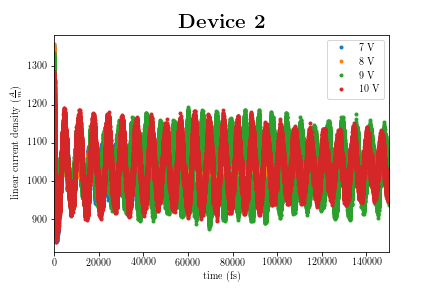
\includegraphics[scale=0.5]{Figures/Device_2/7_to_10V.png}
    \label{fig:dev_2_3}
\end{figure}
\end{frame}

\begin{frame}{Device 2 -- Least Squares Fit}
    \begin{figure}
        \centering
        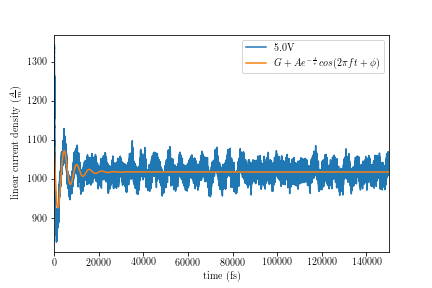
\includegraphics[scale=0.5]{Figures/Device_2/Curve_fit/5_0V.png}
        \label{fig:dev_2_fit}
    \end{figure}
\end{frame}

\begin{frame}{Device 2 -- Channel Voltage vs Steady-State Current}
    \begin{figure}
        \centering
        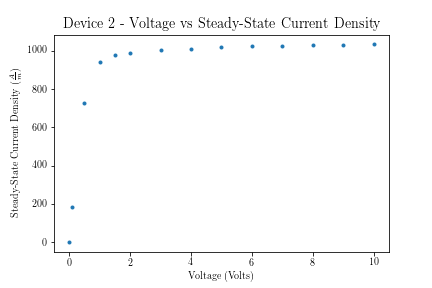
\includegraphics[scale=0.5]{Figures/Device_2/SteadyState.png}
        \label{fig:dev_2_steady}
    \end{figure}
\end{frame}
 
\begin{frame}{Device 3 -- Visual Analysis}

\begin{columns}
\begin{column}{0.5\textwidth}
\begin{figure}
    \centering
    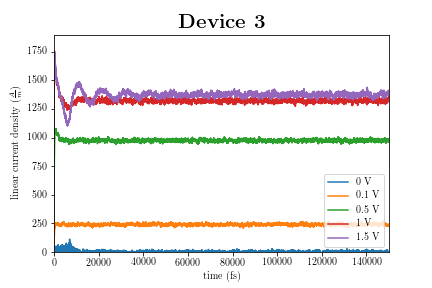
\includegraphics[scale=0.35]{Figures/Device_3/0_to_1_5.png}
    \label{fig:dev_3_1}
\end{figure}{}
\end{column}

\begin{column}{0.5\textwidth}
\begin{itemize}
    \item 0 V, AWGN noise, $\textnormal{mean} = 0 \frac{\textnormal{A}}{\textnormal{m}}$, $\sigma = 7.77 \frac{\textnormal{A}}{\textnormal{m}}$
    \item Response looks second order
    \item Steady-state value with decaying oscillations for $V \leq 1.5 \textnormal{ V}$
    \item Sustained oscillations for $V \geq 2 \textnormal{ V}$
    \item Steady-state saturation at $V \geq 1 \textnormal{ V}$
\end{itemize}
\end{column}
\end{columns}

\end{frame}

\begin{frame}{Device 3 -- Visual Analysis}

\begin{figure}
    \centering
    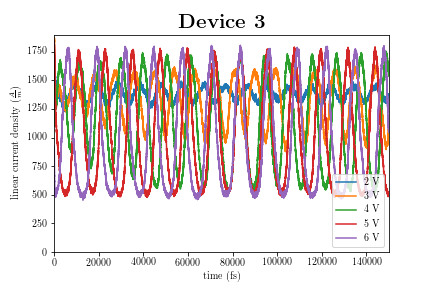
\includegraphics[scale=0.5]{Figures/Device_3/2_to_6V.png}
    \label{fig:dev_3_2}
\end{figure}

\end{frame}

\begin{frame}{Device 3 -- Visual Analysis}
\begin{figure}
    \centering
    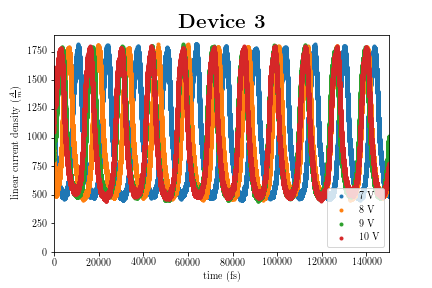
\includegraphics[scale=0.5]{Figures/Device_3/7_to_10V.png}
    \label{fig:dev_3_3}
\end{figure}
\end{frame}

\begin{frame}{Device 3 -- Least Squares Fit}
    \begin{figure}
        \centering
        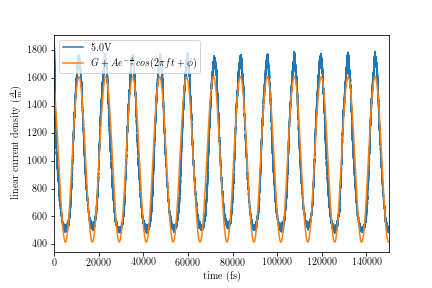
\includegraphics[scale=0.5]{Figures/Device_3/Curve_fit/5_0V.png}
        \label{fig:dev_3_fit}
    \end{figure}
\end{frame}

\begin{frame}{Device 3 -- Channel Voltage vs Steady-State Current}
    \begin{figure}
        \centering
        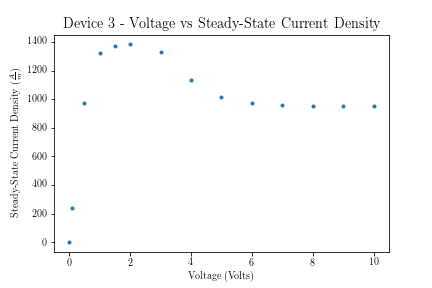
\includegraphics[scale=0.5]{Figures/Device_3/SteadyState.png}
        \label{fig:dev_3_steady}
    \end{figure}
\end{frame}
 
\end{document}